\section{Introduction}
\label{sec:intro}

Symbolic model checking using induction-based techniques such as IC3/PDR~\cite{Bradley11:IC3,Een2011:PDR}, $k$-induction~\cite{SheeranSS00}, and $k$-liveness~\cite{conf/fmcad/ClaessenS12} can often determine whether properties hold of complex finite or infinite-state systems.    Model checking tools are attractive both because they are automated, requiring little or no interaction with the user, and if the answer to a correctness query is negative, they provide a counterexample to the satisfaction of the property.  These counterexamples can be used both to illustrate subtle errors in complex hardware and software designs~\cite{hilt2013,McMillan99:compositional, Miller10:CACM} and to support automated test case generation~\cite{Whalen13:OMCDC, You15:dse}.
In the event that a property is proved, however, it is not always clear what level of assurance should be invested in the result.  Given that these kinds of analyses are performed for safety- and security-critical software, this can lead to overconfidence in the behavior of the fielded system.  Issues such as vacuity~\cite{Kupferman03:Vacuity}, incorrect environmental assumptions~\cite{Whalen07:FMICS}, and errors either in English language requirements or formalization~\cite{Pike06:axioms} can all lead to failures of ``proved'' systems.  Thus, even if proofs are established, one must approach verification with skepticism.

At issue is the level of feedback provided by the tool to the user. In most tools, when the answer to a correctness query is positive, no further information is provided. What we would like to provide is traceability information, a {\em proof core}~ that explains the proof, in much the same way that a counterexample explains the
negative result. This is not a new idea: UNSAT cores~\cite{zhang2003extracting} provide the same kind of information for individual SAT or
SMT queries, and this approach has been lifted to bounded analysis
for Alloy in~\cite{Torlak08:cores} and have been used for hardware model checking~\cite{jasper_gold}. What we propose is a generic and efficient
mechanism for extracting supporting information, similar to an UNSAT
core, from the proofs of safety and liveness properties using inductive techniques
such as PDR and $k$-induction, which we call an {\em inductive validity core} (IVC). Because many properties are not themselves inductive, these proof techniques introduce lemmas as part of the solving process in order to strengthen the properties and make them inductive. Our techniques allow efficient, accurate, and precise extraction of inductive validity cores even in the presence of such auxiliary lemmas.

Once generated, IVCs can be used for many purposes in the software verification process, including at least the following:

\mike{There is something weird with the description environment so I am manually spacing it}

\begin{description}
\item[Vacuity detection:] \quad \quad \quad \quad \quad The idea of syntactic vacuity detection (checking whether all subformulae within a property are necessary for its satisfaction) has been well studied~\cite{Kupferman03:Vacuity}.   However, even if a property is not syntactically vacuous, it may not require substantial portions of the model.  This in turn may indicate that either a.) the model is incorrectly constructed or b.) the property is weaker than expected.  We have seen several examples of this mis-specification in our verification work, especially when variables computed by the model are used as part of antecedents to implications.

\item[Completeness checking:] \quad \quad \quad \quad \quad \quad \quad \ \  
Closely related to vacuity detection is the idea of {\em completeness checking}, e.g., are all atoms in the model necessary for at least one of the properties proven about the model?  Several different notions of completeness checking have been proposed~\cite{chockler_coverage_2003, kupferman_theory_2008}, but these are very expensive to compute, and in some cases, provide an overly strict answer (e.g., checking can only be performed on non-vacuous models for~\cite{kupferman_theory_2008}).

\item[Traceability:] \quad \quad \  
Certification standards for safety-critical systems (e.g.,~\cite{DO178C, MOD:00-55}) usually require {\em traceability matrices} that map high-level requirements to lower-level requirements and (eventually) leaf-level requirements to code or models.  Current traceability approaches involve either manual mappings between requirements and code/models~\cite{SimulinkTraceability} or a heuristic approach involving natural language processing~\cite{Keenan12:Tracelab}.  Both of these approaches tend to be inaccurate.  For functional properties that can be proven with inductive model checkers, inductive validity cores can provide accurate traceability matrices with no user effort.

\item[Symbolic Simulation / Test Case Generation:] \quad \quad \quad \quad \quad \quad \quad \quad \quad \quad \quad \quad \quad \quad \quad \quad \  
Model checkers are now often used for symbolic simulation and structural-coverage-based test case generation~\cite{SimulinkDesignVerifier,Whalen13:OMCDC}.  For either of these purposes, the model checker is supposed to produce a witness trace for a given coverage obligation using a ``trap property'' which is expected to be falsifiable.  In systems of sufficient size, there is often ``dead code'' that cannot ever be reached.  In this case, a proof of non-reachability is produced, and the IVC provides the reason why this code is unreachable.
\end{description}

In addition, it is often the case that there are multiple minimal IVCs (MIVCs) for a given property.  In this case, computing a single MIVC provides, at best, an incomplete picture of the traceability information associated with the proof.  Depending on the model and property to be analyzed, there is often substantial diversity between the IVCs used for proof, and there can also be a substantive difference in the size of a {\em minimal} IVC and a {\em minimum} IVC, which is the (not necessarily unique) smallest MIVC.  If {\em all} MIVCs can be found, then several additional analyses can be performed:

\begin{description}
\item[Coverage Analysis:] \quad \quad \quad \quad \quad 
MIVCs can be used to define coverage metrics by examining the percentage of model elements required for a proof.  However, since MIVCs are not unique, there are multiple, equally legitimate coverage scores possible.  Having \emph{all} MIVCs allows one to define additional metrics: coverage of MAY elements, coverage of MUST elements, as well as policies for the existing MIVC metric: e.g., choose the smallest MIVC. %\ela{I'm not sure if introducing MAY/MUST would make sense to the readers }

\item[Design Optimization:] \quad \quad \quad \quad \quad \quad \ \ \ 
Synthesis tools can benefit from MIVCs in the process of transforming an abstract behavior into a design implementation. A practical way of calculating all MIVCs allows to find a minimum set of design elements (optimal implementation) for a certain behavior. Such optimizations can be performed at different levels of synthesis.

\item[Impact Analysis:] \quad \quad \quad \quad \quad
Given all MIVCs, it is possible to determine which requirements may be falsified by changes to the model.  This analysis allows for selective regression verification of tests and proofs: if there are alternate proof paths that do not require the modified portions of the model, then the requirement does not need to be re-verified.

\item[Robustness Analysis:] \quad \quad \quad \quad \quad \quad
As proposed by Murugesan et. al in~\cite{Murugesan16:renext}, it is possible to partition the model elements into MUST and MAY sets based on whether they are in every MIVC or only some MIVCs, respectively.  This may allow insight into the relative importance of different model elements for the property.  For example, if the MUST set is empty, then the requirement has been implemented in multiple ways, such as would be expected in a fault-tolerant system.
\end{description}

This paper presents a comprehensive explanation of algorithms and applications for inductive validity cores, providing a unified treatment of material from several conference papers~\cite{Ghass16,Murugesan16:renext,Ghass17Cov,Ghass17AllIVCs}, as well as a significantly larger experimental evaluation, revised proofs, and a discussion of {\em granularity} of the model elements on the results produced by IVC algorithms, to provide a definitive treatment of the topic.

%% We put the image here so it shows up side-by-side with fig:ex-after
\begin{figure}[t]
\centering
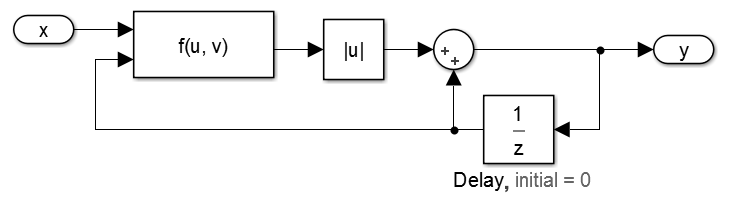
\includegraphics[width=\columnwidth]{figs/simulink.png}
{\smaller
\begin{verbatim}
node filter(x : real) returns (a, b, y : real);
let
  a = f(x, 0.0 -> pre y);
  b = if a >= 0.0 then a else -a;
  y = b + (0.0 -> pre y);
tel;
\end{verbatim}
}
\vspace{-0.1in}
\caption{Model with property $y \geq 0$, before IVC analysis}
\label{fig:ex-before}
\end{figure}

The remainder of the paper is organized as follows... 
